\pdfoutput=1
% In particular, the hyperref package requires pdfLaTeX in order to break URLs across lines.

\documentclass[11pt]{article}

% Change "review" to "final" to generate the final (sometimes called camera-ready) version.
% Change to "preprint" to generate a non-anonymous version with page numbers.
\usepackage[preprint]{acl}

% Standard package includes
\usepackage{times}
\usepackage{latexsym}

% For proper rendering and hyphenation of words containing Latin characters (including in bib files)
\usepackage[T1]{fontenc}
% For Vietnamese characters
% \usepackage[T5]{fontenc}
% See https://www.latex-project.org/help/documentation/encguide.pdf for other character sets

% This assumes your files are encoded as UTF8
\usepackage[utf8]{inputenc}

% This is not strictly necessary, and may be commented out,
% but it will improve the layout of the manuscript,
% and will typically save some space.
\usepackage{microtype}

% This is also not strictly necessary, and may be commented out.
% However, it will improve the aesthetics of text in
% the typewriter font.
\usepackage{inconsolata}

%Including images in your LaTeX document requires adding
%additional package(s)
\usepackage{geometry}
\usepackage{graphicx}
\usepackage{float}
\usepackage{cleveref}
\makeatletter
\AddToHook{cmd/appendix/before}{\def\cref@section@alias{appendix}}
\makeatother

\usepackage{tabularx}             % For flexible-width columns
\usepackage{booktabs}             % For nicer table rules
\usepackage{array}                % Extended col types if needed

% If the title and author information does not fit in the area allocated, uncomment the following
%
%\setlength\titlebox{<dim>}
%
% and set <dim> to something 5cm or larger.

\title{Instructions for *ACL Proceedings}

\usepackage{hyperref}

\makeatletter
\renewcommand{\theHsection}{\thesection}
\renewcommand{\theHsubsection}{\thesubsection}
\renewcommand{\theHsubsubsection}{\thesubsubsection}
\makeatother

\newcommand{\links}{\textbf{\textsc{Links}}}
\newcommand{\recorder}{\textregistered}

\author{%
  My (Chiffon) Nguyen \\
  College of Computational Sciences \\
  Minerva University \\
  San Francisco, CA 94108 \\
  chiffonng@uni.minerva.edu
}

\begin{document}

\begin{titlepage}
\centering
{\scshape\LARGE Minerva University \par}
\vspace{1cm}
\begin{center}
    
\includegraphics[width = 0.4\linewidth]{figures/minerva_logo.png}
\end{center}
{\scshape\Large Capstone: Class of 2025 \par}
\vspace{1.5cm}
{\huge\bfseries LINKS: Generate linguistically grounded mnemonic devices for English vocabulary learning with reasoning, multilingual LLMs \par}
\vspace{2cm}
{\scshape\large Tra My Nguyen \par}
submitted in partial fulfillment of the requirements for the degree of Bachelor of Science in Computational Sciences \par
\vspace{2cm}
{\large\itshape Capstone Committee \par}
Dr. Patrick Watson \\
Dr. Philip Sterne

\vfill
{\large \today\par}
\end{titlepage}

\onecolumn
\section*{Executive Summary}
Note: Due to limited compute, some experiments conducted are small-scale and need more data for robust validation and conclusion. However, the codebase is reproducible and scalable when there is more compute.

Tags: computational linguistics, natural language processing, large language model, language education, english as a foreign language, vocabulary acquisition, synthetic data generation.

\clearpage

\tableofcontents
\clearpage

\twocolumn

\maketitle
\begin{abstract}
To acquire advanced vocabulary, English learners often use mnemonic devices, memorable associations linking a new concept to learned concepts to improve memory and recall. Reviewing the literature on mnemonic techniques, we characterize good mnemonics as \textbf{linguistically grounded}, which better link to the target vocabulary, improving long-term retention and linguistic knowledge, especially at advanced levels (CEFR B2+). We investigate whether Large Language Models can consistently help write such effective mnemonics, with three different settings: in-context learning, and reasoning distillation. Concretely, we first measured different prompting strategies with a frontier reasoning model, DeepSeek-R1, and generated \links, a synthetic dataset of 2000 triplets of \textit{reasoning trace, mnemonic, and example sentence} for 2000 vocabulary useful for TOEFL iBT \footnote{Internet-based Test of English as a Foreign Language}, IELTS Academic \footnote{International English Language Testing System}, and SAT\footnote{Scholastic Aptitude Test}. Second, using a subset of \links, we distilled linguistic reasoning from the \textit{teacher model} to the \textit{student model}, Gemma-3-1b-it\footnote{https://huggingface.co/collections/google/gemma-3-release-67c6c6f89c4f76621268bb6d} , with online reinforcement learning. The trained, quantized model can be served with a local application such as OpenWebUI (interface) and Ollama (command-line).

Preliminary evaluation shows

The project examplifies that carefully designed NLP systems can generate resources for language learning, either in classroom settings or in self-study. Code, models, and dataset are available\footnote{Links: \href{https://github.com/chiffonng/mnemonic-gen}{Github codebase} and \href{https://huggingface.co/collections/chiffonng/vocab-mnemonic-mining-67563a0a1ab91e84e9827579}{HuggingFace collection of datasets and artifacts}}.
\end{abstract}

\section{Introduction}
Vocabulary acquisition challenges many English language learners, particularly at upper intermediate to advanced levels where abstract and academic vocabulary predominates. Mnemonics, cognitive tools that help learners create associations between new vocabulary and familiar concepts, serve as valuable tools for enhancing retention and recall. The deeper learners elaborate the connection between the mnemonic and the target vocabulary, the longer and better they can recall the term \citealp{}. However, creating such effective mnemonics demands both linguistic expertise and creative effort, presenting a significant barrier for most learners. Large Language Models (LLMs) have demonstrated capabilities as knowledge bases and creative text generators, suggesting their potential for automated mnemonic generation.

Previous work explored automated mnemonic generation through computational methods using the \textbf{keyword method}, which involves 1) generateing simpler keywords that together sound or look like the target vocabulary and 2) creating memorable explanations that include the vocabulary, the keywords, amd its meaning \citep{atkinsonApplicationMnemonicKeyword1975}. \citet{savvaTransPhonerAutomatedMnemonic2014} and \citet{OzbalAUTOMATION2014} generated keywords of phonetic and orthographic similarities in the native language for foreign language vocabulary, across multiple languages. \citet{LeeSMARTPHONE2023} extended this work and utilized LLMs to produce phonetically similar keywords and visual cues and \citet{LeeEXPLORING2024} prompted LLMs to generate multiple mnemonic candidates and evaluate them based on imageability and coherence. Most recently, \citet{balepurSMART2024} fine-tuned LLaMA-2-70B on 800 crowd-sourced mnemonics and aligned outputs with learner preferences and learning outcomes.

%%%% Figure Highlight the difference between keyword "mnemonic" and "linguistically grounded mnemonics" with an example
%%% (e.g., \textbf{preposterous} can be broken down as pre- (before) + poster (after) + ous. Anything that comes both before and after is preposterous)

Although the keyword method is commonly used and empirically validated in classroom and laboratory contexts \citetext{\citealp{atkinsonApplicationMnemonicKeyword1975}, \citealp{pressleyMnemonicKeywordMethod1982}}, it may lead to longer retrieval time \citep{vanhellKeywordMnemonicsRote1997} and be inadequate for fairly abstract vocabulary \citetext{\citealp{camposLimitationsMnemonicKeywordMethod2003}, \citealp{camposImportanceKeywordGenerationMethod2004a}}. Such methods typically neglect other rich linguistic knowledge embedded in LLMs that could provide diverse mnemonic strategies beyond simple keyword associations. Second, previous works passively deliver generated mnemonics to learners. While \textsc{Smart} \citep{balepurSMART2024} was further trained on learners' preferences, these preferences were aggregated, potentially missing alignment with individual learning styles. Language learners who use self-created mnemonics retain vocabulary more effectively and for longer duration \citep{madanExploringWordMemorability2021}.


Contributions:

Generate diverse linguistically grounded mnemonics to learn and memorize the meaning and writing of English vocabulary, through prompting LLMs. Our method overcomes LLMs pre-training biases, e.g. associated with the word “mnemonic” by using synthetic chain-of-thought reasoning on linguistic features of the vocabulary and few-shot structured examples.

Impart the linguistic reasoning and creative writing style to smaller models like Gemma 3 through fine-tuning on synthetic CoT data in the first step.

\section{Background}
\subsection{Mnemonic devices for vocabulary learning}

\begin{table*}[htb] \label{tab:linguistic-features}
\centering
\caption{Examples of feature categories for English words.}
\label{tab:features}
\begin{tabularx}{\textwidth}{l >{\raggedright\arraybackslash}X >{\raggedright\arraybackslash}X}
\toprule
\textbf{feature} & \textbf{description} & \textbf{example} \\
\midrule
\textbf{phonetics} & vocab's sound patterns & \emph{apparent} sounds like “a bare Asian.” \\
\addlinespace
\textbf{orthography} & written/spelling patterns & \emph{abet} looks like “a + bet.” \\
\addlinespace
\textbf{morphology} & structure including free and bound morphemes & \emph{aggrandize} = a + grand + –ize \\
\addlinespace
\textbf{etymology} & vocab origin & \emph{adumbrate} comes from Latin \emph{umbra} \\
\addlinespace
\textbf{semantics} & vocab meaning and relationships & \emph{confound} is similar to “confuse.” \\
\bottomrule
\end{tabularx}
\end{table*}

\section{In-context learning performance} \label{sec:icl-performance}
We systematically compared various in-context learning approaches to understand how different prompting techniques affect mnemonic generation. \Cref{fig:prompting-methods} illustrates the percentage of linguistically grounded mnemonics generated by different prompt formulations. Given the importance of the explanation connecting the vocabulary with the actual mnemonic, we experimented with reasoning LLMs.


\begin{figure}
  \centering
  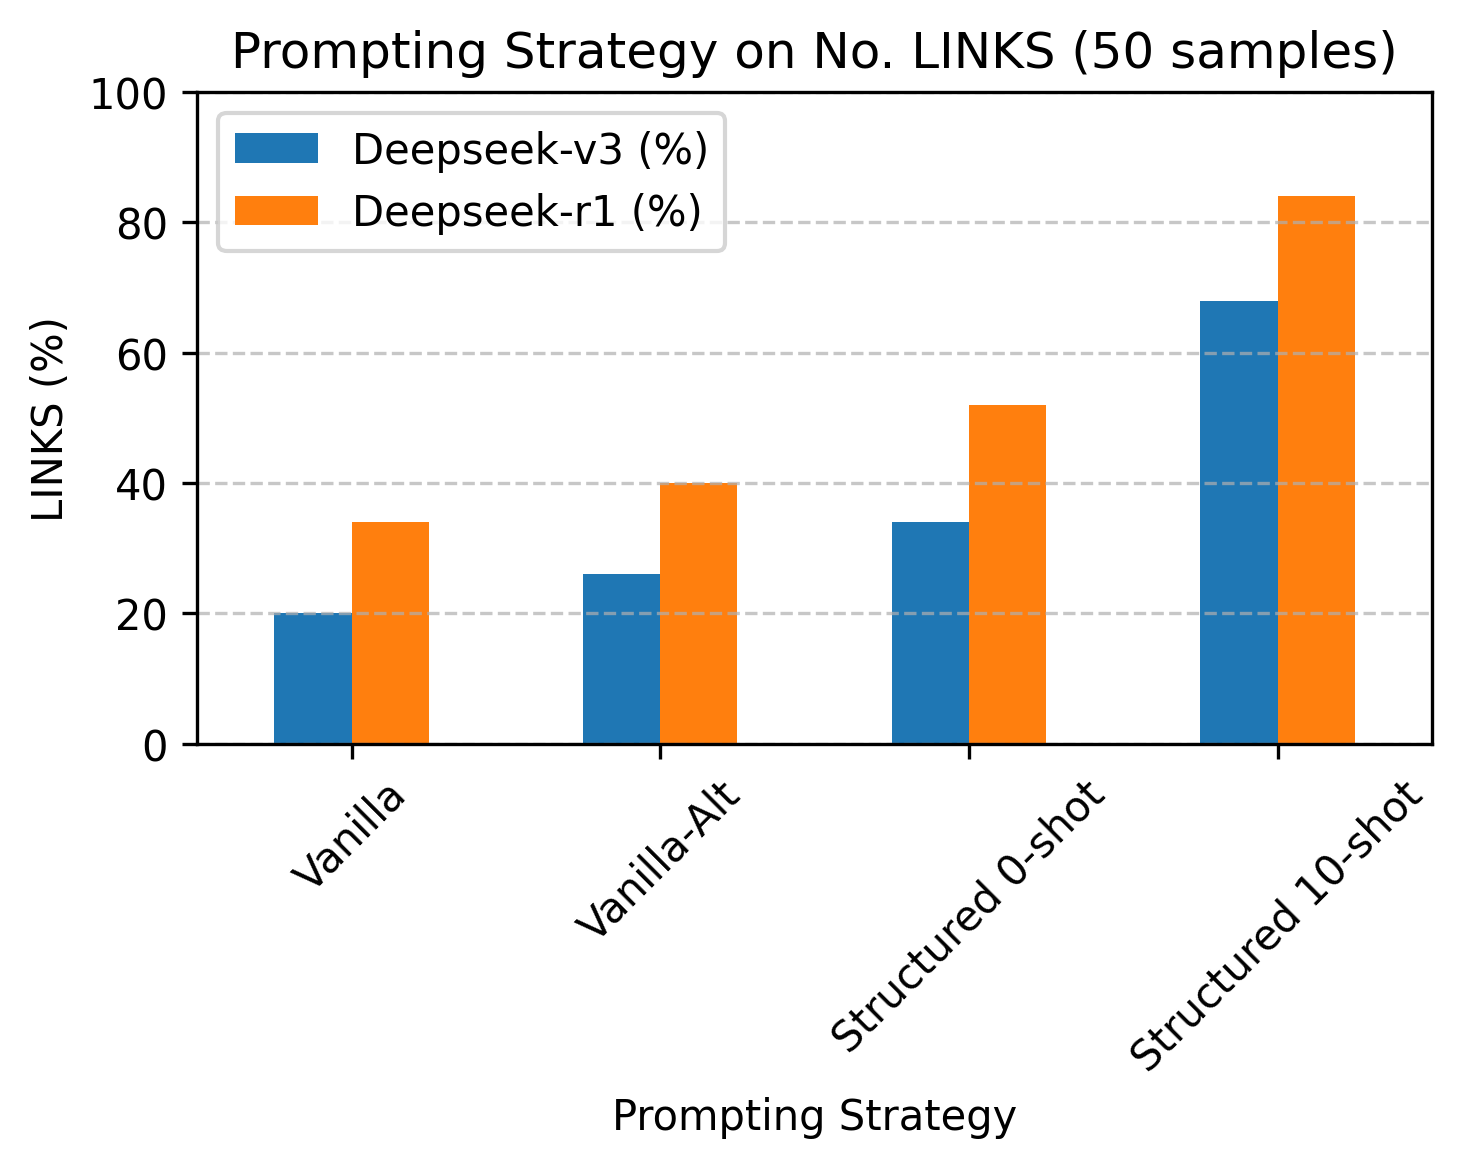
\includegraphics[width=\linewidth]{figures/prompt_comparison.png}
  \caption{Comparison of prompting methods (see detailed prompt in \Cref{app:prompt-usage}). Y-axis shows percentages of linguistically-grounded mnemonics generated out of 50 requests sent for each prompt type.}
  \label{fig:prompting-methods}
\end{figure}

We observed significant variation in the quality and linguistic grounding of generated mnemonics based solely on prompt formulation. Four distinct prompting strategies were evaluated (see details in \cref{app:prompt-usage})
Vanilla
Reasoning LLMs tend to overthink \citep{xuChainDraftThinking2025}
Good practices: provide decomposed instructions, structured output format, demonstration examples \citep{MishraREFRAMING2022}, and clarify definitions of linguistic features \citep{yinDidYouRead2023}

compress task definition \citep{yinDidYouRead2023},


\section{Knowledge and reasoning distillation}


\subsection{Data construction}
\citep{longLLMsDrivenSyntheticData2024b}

\subsection{Training and inference}


\section{Evaluation}
\subsection{Experimental setup}

\paragraph{LLM-as-a-judge for 1-5 Likert ratings}

\paragraph{Pairwise preference using double-blind annotation}

\paragraph{Interactive side-by-side comparison}

\subsection{Results}

\section{Related work}
\section{Discussion}
\section{Conclusion}
\section{Limitations}

\section*{Acknowledgements}
% Bibliography entries for the entire Anthology, followed by custom entries
\bibliography{custom}
% Custom bibliography entries only
%\bibliography{anthology,custom}

\clearpage
\appendix

\section{Detailed prompt usage} \label{app:prompt-usage}

All of the prompts include

\paragraph{Vanilla vs. Alternative Phrasing} When comparing "Generate a mnemonic to help learn and remember the meaning of English vocabulary and how it is written: \{term\}" against "Generate a memory cue to help learn and remember the meaning of English vocabulary and how it is written: \{term\}", we observed substantial differences in output quality. This highlights the word importance effect noted by \citet{hackmannWordImportanceExplains2024}, where specific terms like "mnemonic" may have acquired pre-training biases that associate them primarily with acronyms or keyword methods rather than broader linguistic strategies.

\paragraph{Structured Prompting} We found improved performance with structured prompts that explicitly request linguistic analysis: "Generate a linguistically grounded mnemonic to help me learn and remember the meaning of English vocabulary and how it is written: \{term\}. Think in short traces and stop when you have a good linguistic connection. You must use that linguistic feature to form a mnemonic for the word." This approach yielded a higher percentage of mnemonics with clear linguistic association.

\paragraph{Chain-of-Thought (CoT) Prompting} Incorporating chain-of-thought reasoning by providing both the instruction and examples of step-by-step linguistic analysis significantly improved the quality of generated mnemonics. Our implementation used 10 human-written examples, each demonstrating the process of finding linguistic association of the vocabulary before constructing a mnemonic.

\paragraph{Concise Reasoning Traces} Inspired by \citet{xuChainDraftThinking2025}, we experimented with prompting models to generate minimal reasoning steps. For example: "Generate a mnemonic for \{term\}. Think step by step, but keep a minimum draft for each thinking step." This approach balanced comprehensive linguistic analysis with efficiency, preventing models from overthinking and/or elaborating on irrelevant aspects.


\section{Annotation details} \label{app:annotation}

\subsection{}

\section{Documentation of previous iterations}
\subsection{Fine-tuning with OpenAI}

\subsection{Fine-tuning with Gemma-3-4b-it}


\end{document}
